We now know what objects people remember and the factors that influence their memorability, but to what extent does the memorability of individual objects affect the overall memorability of a scene? Moreover, if an image is highly memorable, what can we say about the memorability of the objects inside those images (and vice versa)? To shed light on this question, we conducted a second large-scale experiment on Amazon Mechanical Turk for all images in our dataset to gather their respective image memorability scores. For this experiment, we followed the exact paradigm as the memory game experiment proposed in \cite{isola11}. [add details about the fillers, add details about the experiment including number of workers, number of times each image was viewed by workers and explain the consistency analysis]

Utilizing results from both experiments, we computed the correlation between the the scores of the single most memorable object in each image (from Experiment 1) and the overall memorability score of each image (from Experiment 2). We found this correlation to be moderately high ($\rho=0.4$), suggesting that the most highly memorable object in the image plays a crucial role in determining the overall memorability of an image. To investigate this finding in relation to extreme cases only, we performed the same analysis as above on a subset of the data containing the topmost $100$ memorable images and the bottommost $100$ memorable images. The correlation between maximum object memorability and image memorability for this subset of the images increased significantly ($\rho=0.62$), meaning maximum object memorability serves as a strong indicator of whether an image is \textit{highly} memorable or non-memorable. That is, images that are highly memorable contain at least one highly memorable object, and images with low memorability usually do not contain a single highly memorable object [refer to qual figure].

It seems that maximum object memorability is highly explanatory, but does this behavior generalize across object classes? We further computed the correlation between maximum object and image memorability for each individual object class. Results shown in  Table \ref{tab:tableMem} show that certain object classes are more strongly correlated than others.  For example, images containing animals, buildings, or vehicles as the most memorable objects tend to have varying degree of image memorability (indicated by their lower $\rho$ values). On the other hand, classes like device, furniture, nature, and person are strongly correlated with image memorability, indicating that if an image’s most memorable object belongs to one of these classes, the object memorability score is strongly predictive of the image memorability score. We can imagine scenarios in which this information would be useful. For example, in the case where vision systems are tasked to predict scene memorability, a \textit{single} object and it’s class can serve as a strong prior in predicting image memorability.

\begin{table}[b]
    \begin{tabular}{cccccccc}
    \hline
    Animal & Building & Device & Furniture & Nature & Person & Vehicle & All  \\ \hline
    0.38   & 0.22     & 0.47   & 0.53      & 0.64   & 0.54   & 0.30    & 0.40 \\ \hline
    \end{tabular}
    \caption{\footnotesize\textbf{Max object memorability and image memorability.} add-in later. }\label{tab:tableMem}
\end{table}


\begin{figure*}[!b]
\centering
\subfigure{\centering 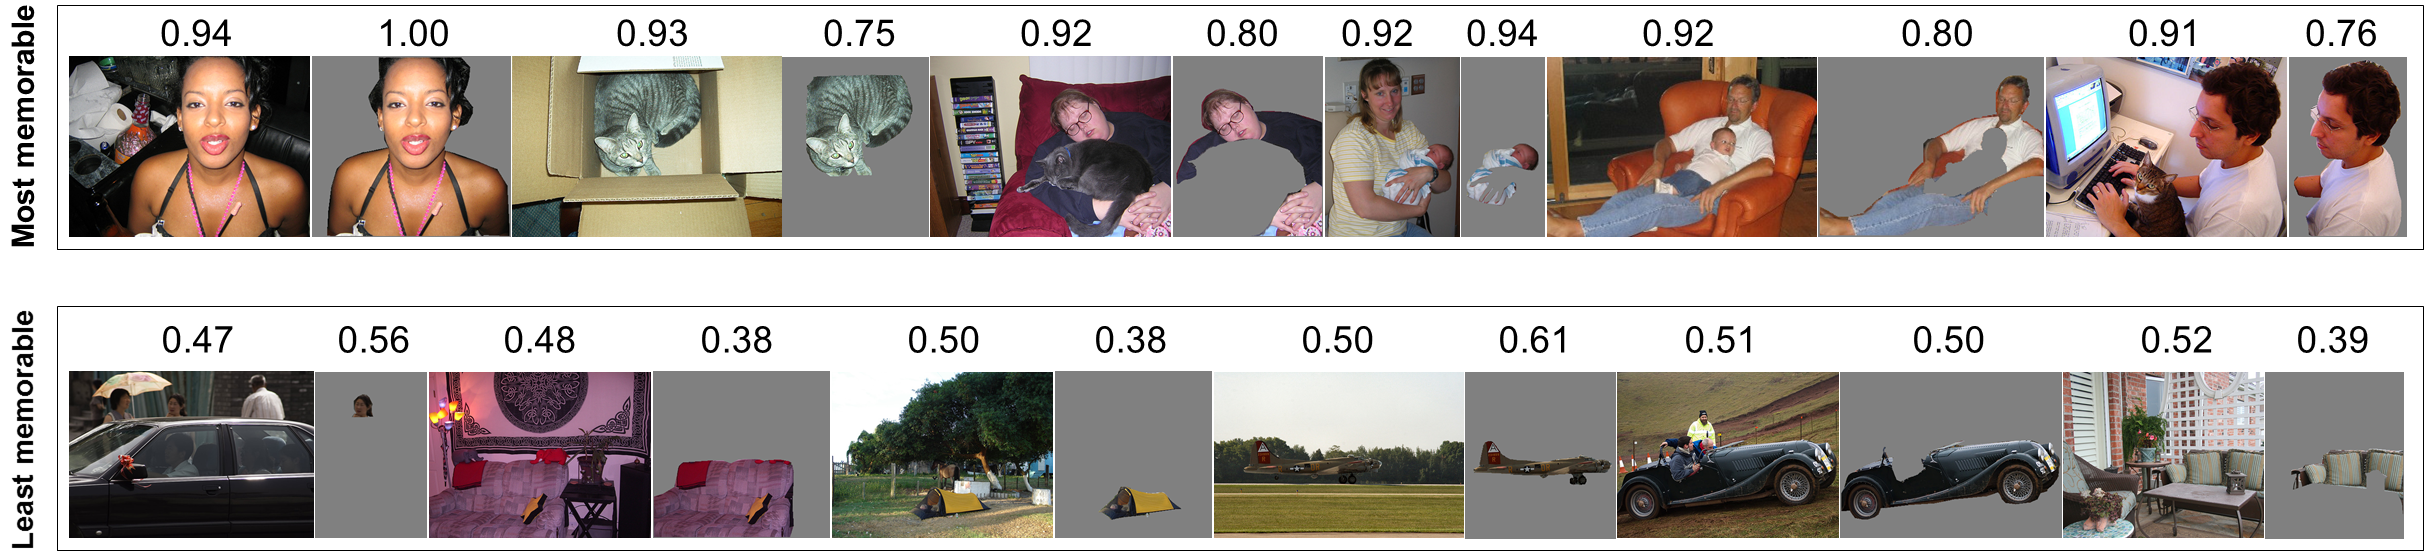
\includegraphics[width=1\textwidth]{figures/results/imMem/qual.png}}
\vspace{-5mm}\caption{\footnotesize\textbf{Qual image-object results.} add-in later. }\label{fig:imMemQual}
\end{figure*}



